\section{Výstupní data}
Výstupní data obsahují body obarvené podle clusterů, ke kterým patří. U algoritmu K-means byly navíc černě vykresleny centroidy vypočítané vlastní implementací algoritmu a červeně centroidy určené integrovanou funkcí \texttt{kmeans} v MATLABu. Tato vizualizace umožňuje porovnat přesnost a odlišnosti obou přístupů.

\subsection{Jednorozměrná data}

\begin{figure}[H]
    \centering
    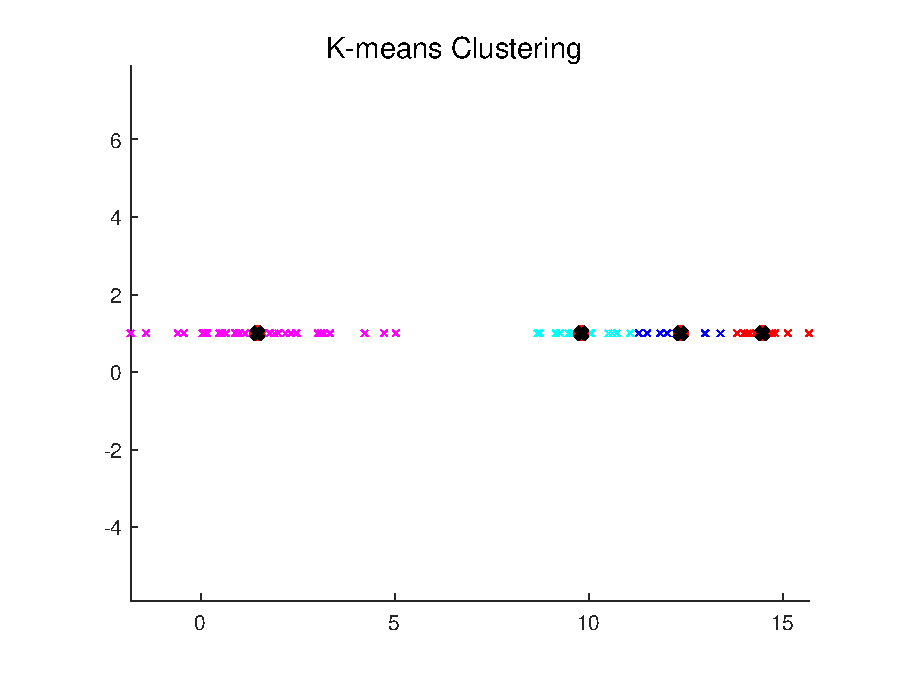
\includegraphics[width=0.5\textwidth]{images/1D_kmeans_2.eps}
    \caption{K-means pro jednorozměrná data.}
\end{figure}

\begin{figure}[H]
    \centering
    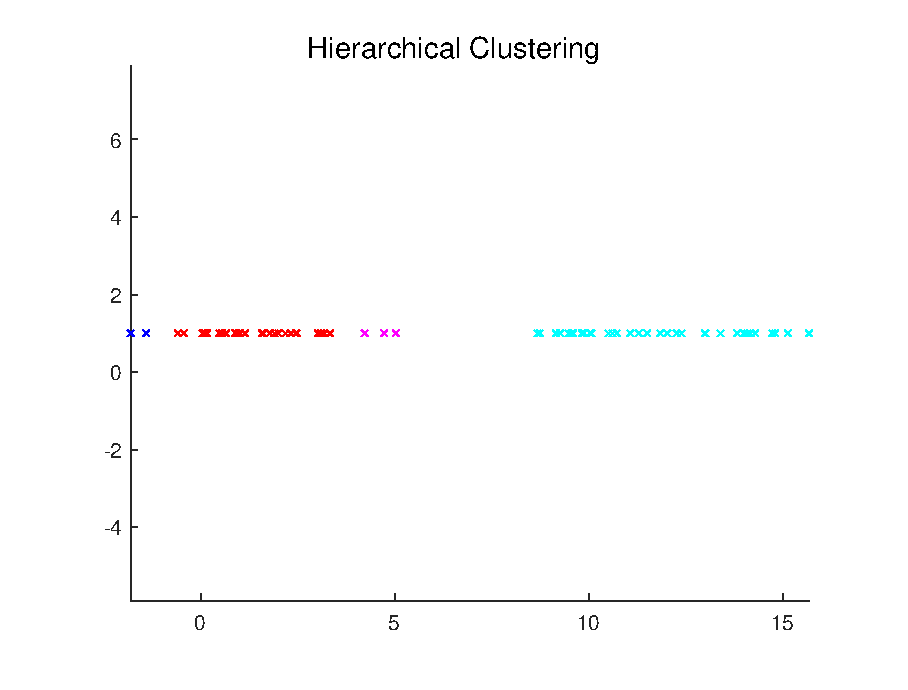
\includegraphics[width=0.5\textwidth]{images/1D_hierar_2.eps}
    \caption{Hierarchické shlukování pro jednorozměrná data.}
\end{figure}

\begin{figure}[H]
    \centering
    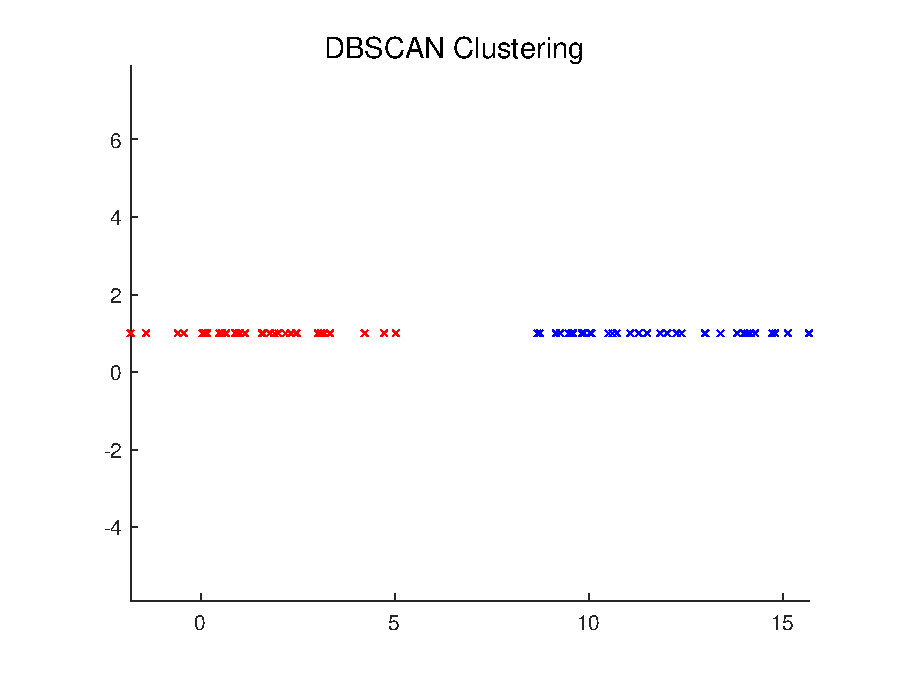
\includegraphics[width=0.5\textwidth]{images/1D_DBSCAN_2.eps}
    \caption{DBSCAN pro jednorozměrná data.}
\end{figure}

\subsection{Dvourozměrná data}

\begin{figure}[H]
    \centering
    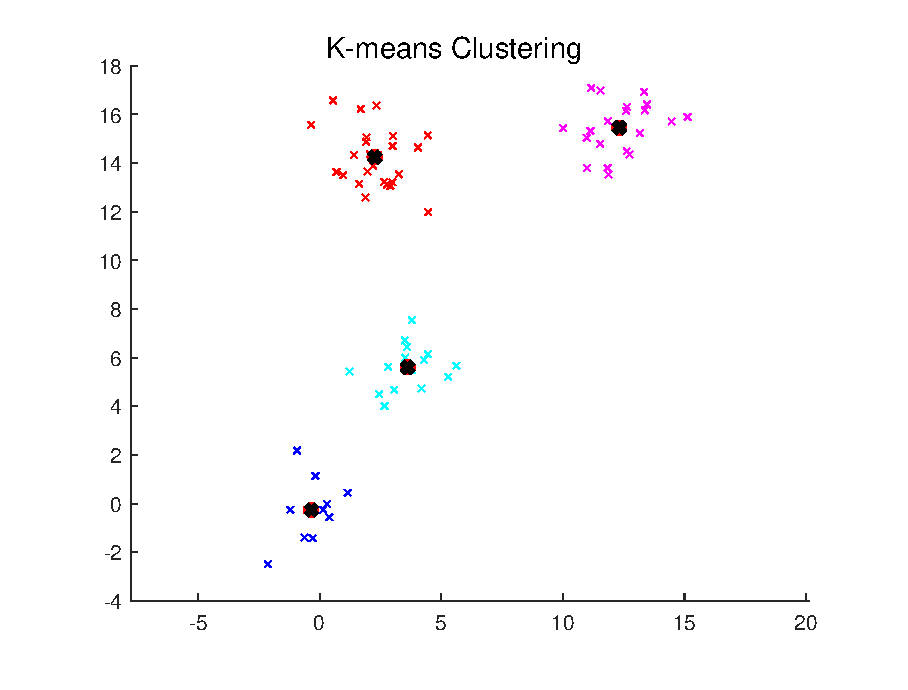
\includegraphics[width=0.5\textwidth]{images/2D_kmeans.eps}
    \caption{K-means pro dvojrozměrná data.}
\end{figure}

\begin{figure}[H]
    \centering
    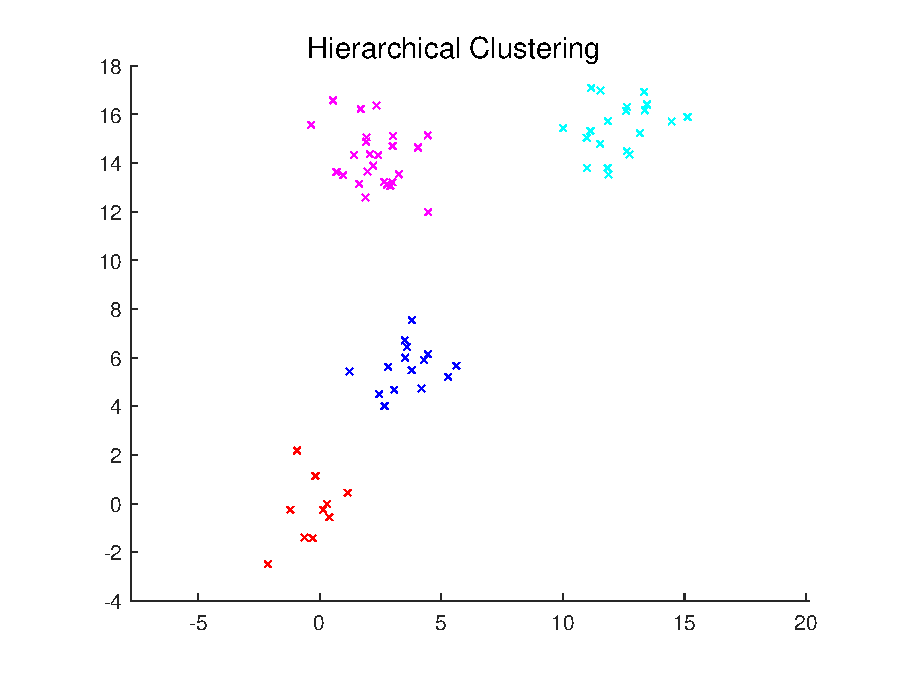
\includegraphics[width=0.5\textwidth]{images/2D_hierar.eps}
    \caption{Hierarchické shlukování pro dvojrozměrná data.}
\end{figure}

\begin{figure}[H]
    \centering
    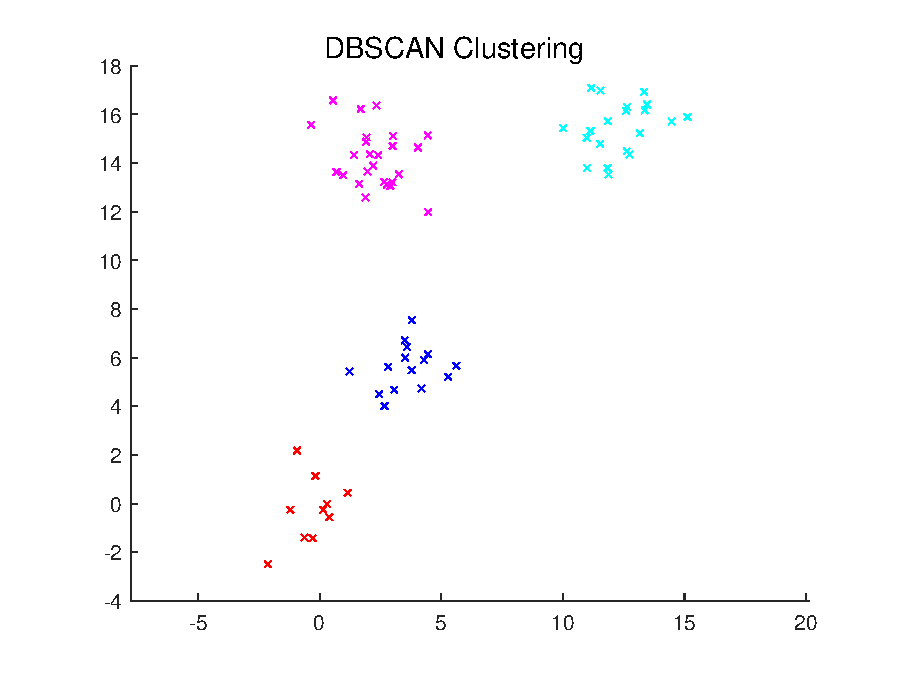
\includegraphics[width=0.5\textwidth]{images/2D_DBSCAN.eps}
    \caption{DBSCAN pro dvojrozměrná data.}
\end{figure}

\subsection{Trojrozměrná data}

\begin{figure}[H]
    \centering
    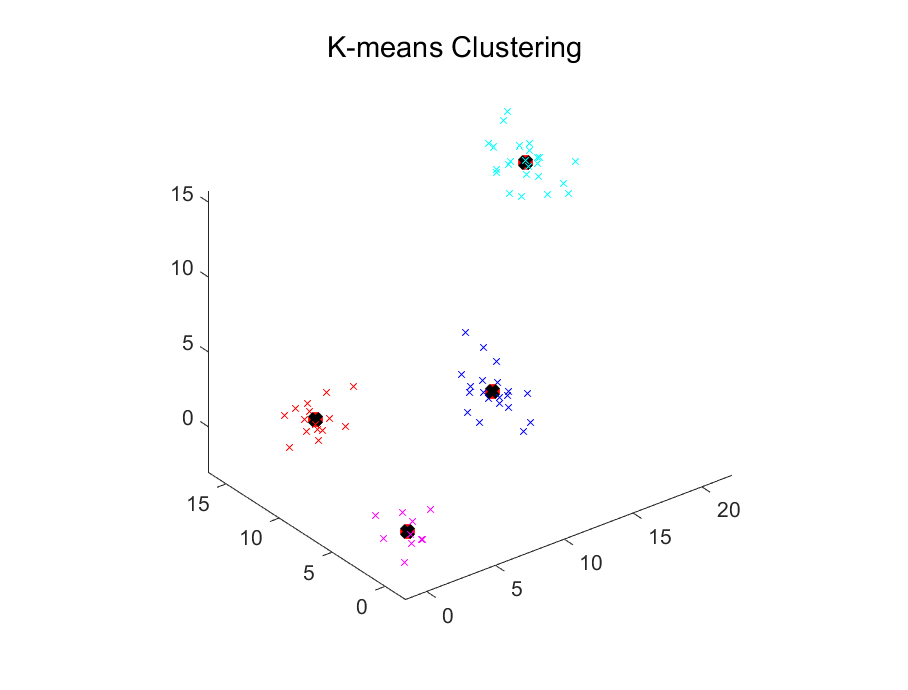
\includegraphics[width=0.5\textwidth]{images/3D_kmeans.eps}
    \caption{K-means pro trojrozměrná data.}
\end{figure}

\begin{figure}[H]
    \centering
    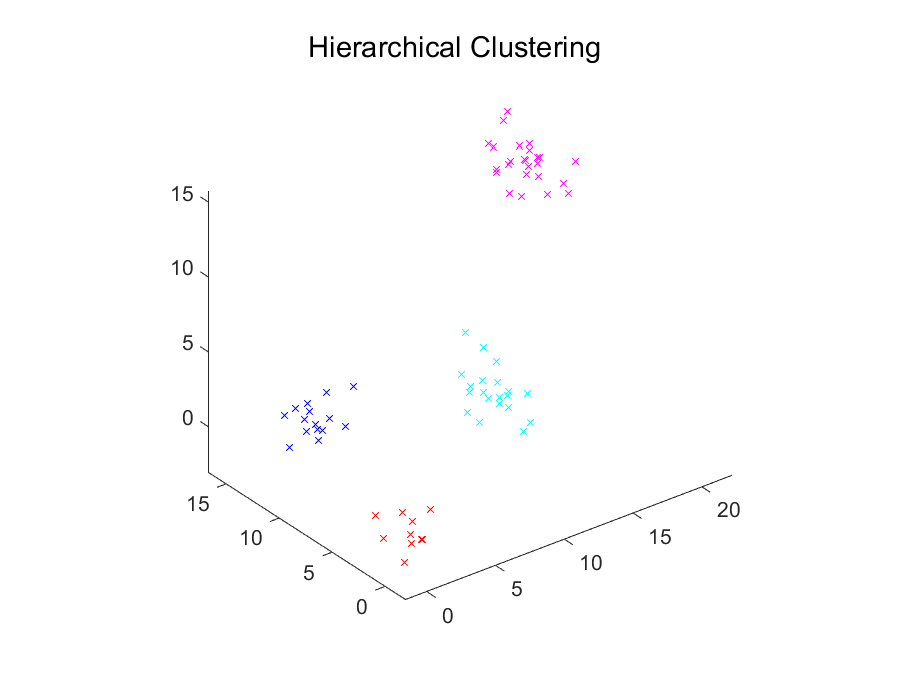
\includegraphics[width=0.5\textwidth]{images/3D_hierar.eps}
    \caption{Hierarchické shlukování pro trojrozměrná data.}
\end{figure}

\begin{figure}[H]
    \centering
    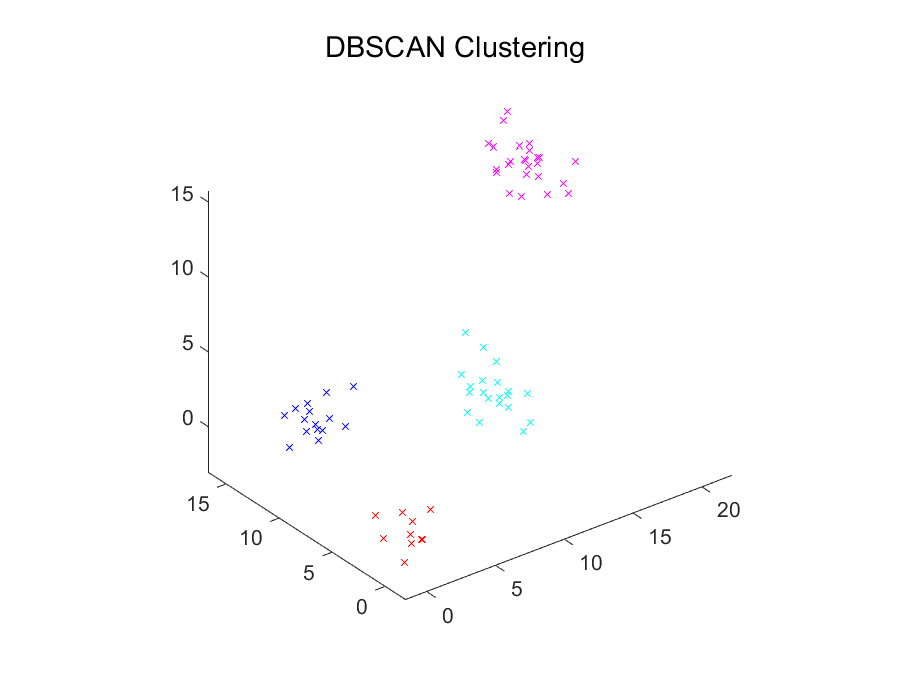
\includegraphics[width=0.5\textwidth]{images/3D_DBSCAN.eps}
    \caption{DBSCAN pro trojrozměrná data.}
\end{figure}

\subsection{Čtyřrozměrná data}

\begin{figure}[H]
    \centering
    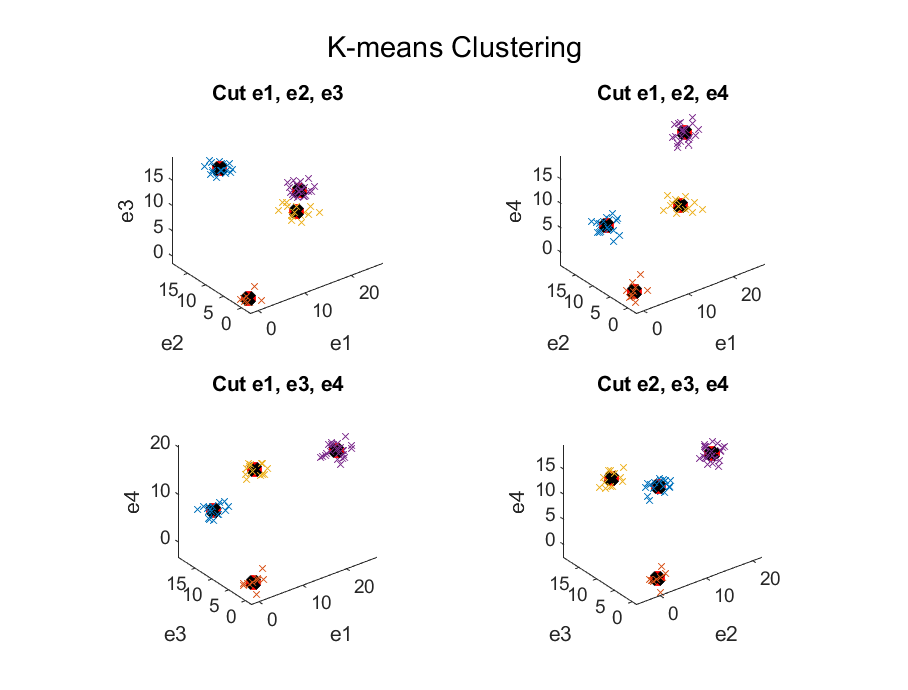
\includegraphics[width=0.5\textwidth]{images/4D_kmeans.eps}
    \caption{K-means pro čtyřrozměrná data.}
\end{figure}

\begin{figure}[H]
    \centering
    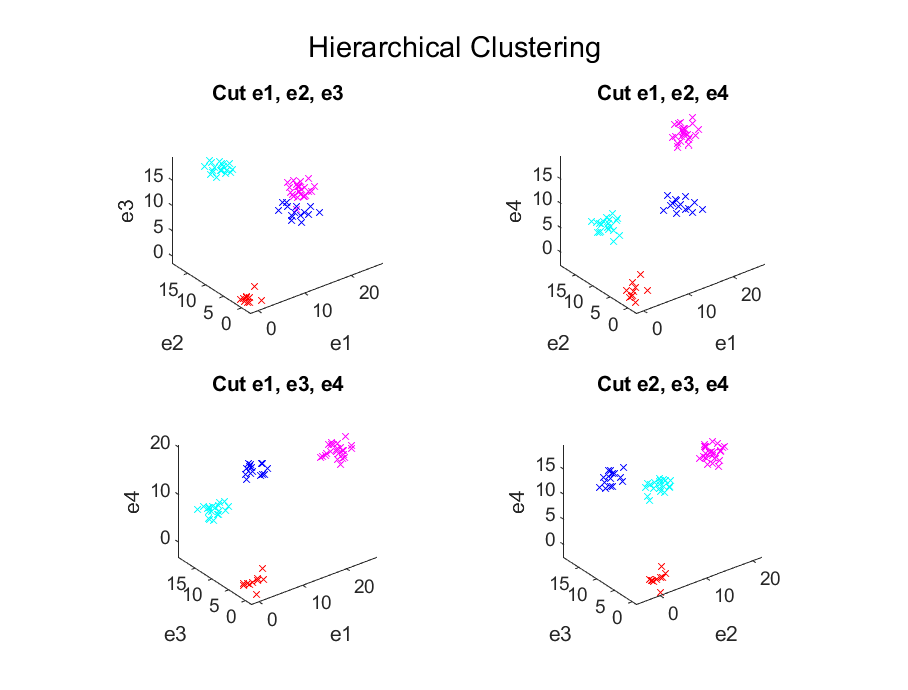
\includegraphics[width=0.5\textwidth]{images/4D_hierar.eps}
    \caption{Hierarchické shlukování pro čtyřrozměrná data.}
\end{figure}

\begin{figure}[H]
    \centering
    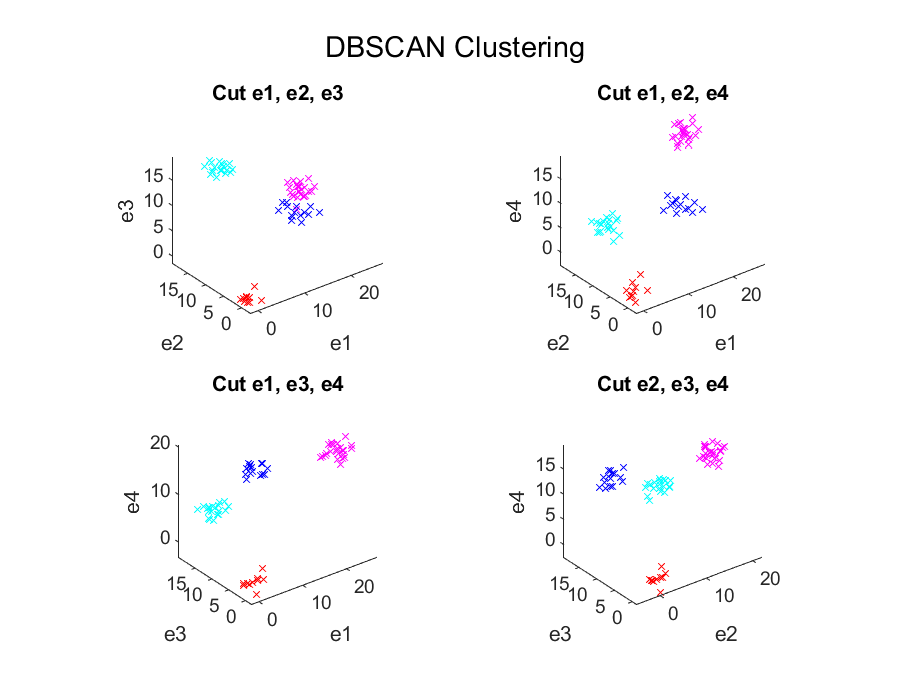
\includegraphics[width=0.5\textwidth]{images/4D_DBSCAN.eps}
    \caption{DBSCAN pro čtyřrozměrná data.}
\end{figure}

\subsection{Rozdílný výsledek K-means}
V některých případech se výsledky vlastní implementace K-means a implementace v MATLABu liší. Tento rozdíl je pravděpodobně způsoben náhodnou inicializací centroidů při startu algoritmu.

\begin{figure}[H]
    \centering
    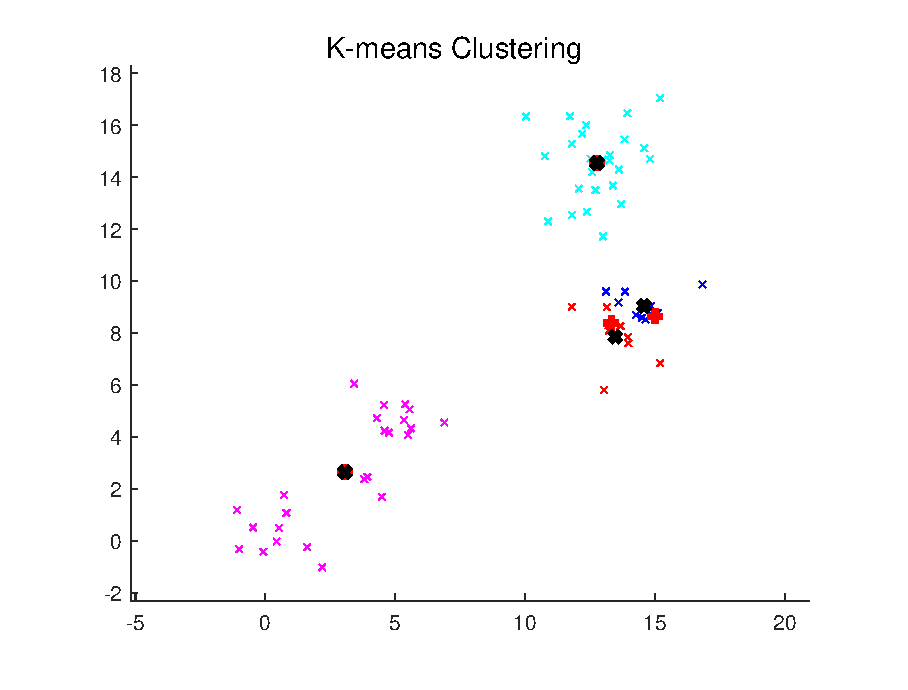
\includegraphics[width=0.65\textwidth]{images/kmeans_difference.eps}
    \caption{Rozdíly mezi vlastní implementací a MATLAB implementací K-means.}
\end{figure}
